\documentclass[border=12pt]{standalone}
\def\pgfsysdriver{pgfsys-dvisvgm.def}
\usepackage[dvisvgm]{xcolor}
\usepackage{xeCJK}
\setCJKmainfont{HaranoAjiGothic-Regular.otf}[BoldFont=HaranoAjiGothic-Bold.otf]
\setCJKsansfont{HaranoAjiGothic-Regular.otf}[BoldFont=HaranoAjiGothic-Bold.otf]
\usepackage{amsmath,amssymb,tikz,lmodern}
\usetikzlibrary{arrows.meta,positioning,calc,fit,backgrounds}
\renewcommand{\familydefault}{\sfdefault}
\definecolor{ink}{HTML}{25322F}
\definecolor{green}{HTML}{246657}
\definecolor{tint}{HTML}{EEF4F0}
\definecolor{soft}{HTML}{C6D2CC}
\definecolor{muted}{HTML}{52615B}
\newif\ifJapanese
\newcommand{\Tx}[2]{\ifJapanese #1\else #2\fi}
\newcommand{\Eff}{\overline{\operatorname{Eff}}}
\newcommand{\heading}[3]{{\color{green}\bfseries #1\quad\Tx{#2}{#3}}\\[5pt]}
% A white rectangle makes the complete citation label clickable, including spaces.
\newcommand{\refurl}[2]{\special{dvisvgm:raw <a xlink:href="#1" target="_blank" rel="noopener noreferrer">}{\setlength{\fboxsep}{0pt}\colorbox{white}{\color{green}\underline{\strut #2}}}\special{dvisvgm:raw </a>}}
\newcommand{\refedge}[3]{\refurl{\csname source#1\endcsname\string##page=#2}{#3}}
\newcommand{\SF}[2]{\refedge{sf}{#1}{#2}}
% GitHub's file preview does not support PDF page fragments.
\newcommand{\LA}[2]{\refurl{\sourcela}{#2}}
\newcommand{\Sch}[2]{\refedge{sch}{#1}{#2}}
\newcommand{\PS}[2]{\refedge{ps}{#1}{#2}}
\tikzset{
 card/.style={draw=soft,fill=white,rounded corners=2pt,align=left,text=ink,font=\fontsize{10.5}{14}\selectfont,inner xsep=12pt,inner ysep=10pt,text width=14.4cm},
 half/.style={card,text width=6.45cm,minimum height=2.05cm},
 result/.style={card,draw=green,fill=tint,line width=.9pt},
 reason/.style={align=left,text=muted,font=\fontsize{9}{12}\selectfont,inner sep=0pt,text width=12.7cm},
 branchreason/.style={reason,text width=5.95cm},
 edge/.style={-{Stealth[length=2.4mm]},draw=green,line width=1pt},
 wire/.style={draw=green,line width=1pt},
}
% Keep the arrow in a dedicated left gutter; explanations never cover it.
\newcommand{\flow}[3]{
 \coordinate (#2-from) at ($(#1.south)+(-6.9,0)$);
 \coordinate (#2-to) at ($(#2.north)+(-6.9,0)$);
 \draw[edge] (#2-from)--(#2-to);
 \node[reason,anchor=west] (#2-reason) at ($(#2-from)!.5!(#2-to)+(.55,0)$) {#3};
}

\newcommand{\Hash}[2]{\refurl{\sourcehash}{#2}}
\newcommand{\FGring}[2]{\refedge{rings}{#1}{#2}}
\newcommand{\FGglue}[2]{\refedge{glue}{#1}{#2}}
\newcommand{\OI}[2]{\refurl{\sourceoi}{#2}}

\Japanesefalse
\newcommand{\sourcela}{https://github.com/openai/math/blob/adc7f1241b42e322a6451854ab7e4b4c146bf78a/preprints/Log-abundance-in-characteristic-zero-September-24-2026/paper.pdf}
\newcommand{\sourcehash}{https://arxiv.org/html/1609.00121v4}
\newcommand{\sourceglue}{https://www.math.kyoto-u.ac.jp/~fujino/fg-comp-final.pdf}
\newcommand{\sourcerings}{https://www.math.kyoto-u.ac.jp/~fujino/log-ring-aspm.pdf}
\newcommand{\sourceoi}{https://github.com/openai/math/blob/adc7f1241b42e322a6451854ab7e4b4c146bf78a/preprints/Orbifold-and-logarithmic-Iitaka-subadditivity-September-26-2026/paper.pdf}
\newcommand{\sourcehps}{https://people.math.harvard.edu/~mpopa/papers/HPS.pdf}
\newcommand{\sourcegmm}{https://github.com/openai/math/blob/adc7f1241b42e322a6451854ab7e4b4c146bf78a/preprints/Minimal-models-and-Mori-fibre-spaces-for-generalized-log-canonical-Q-pairs-September-24-2026/paper.pdf}
\begin{document}
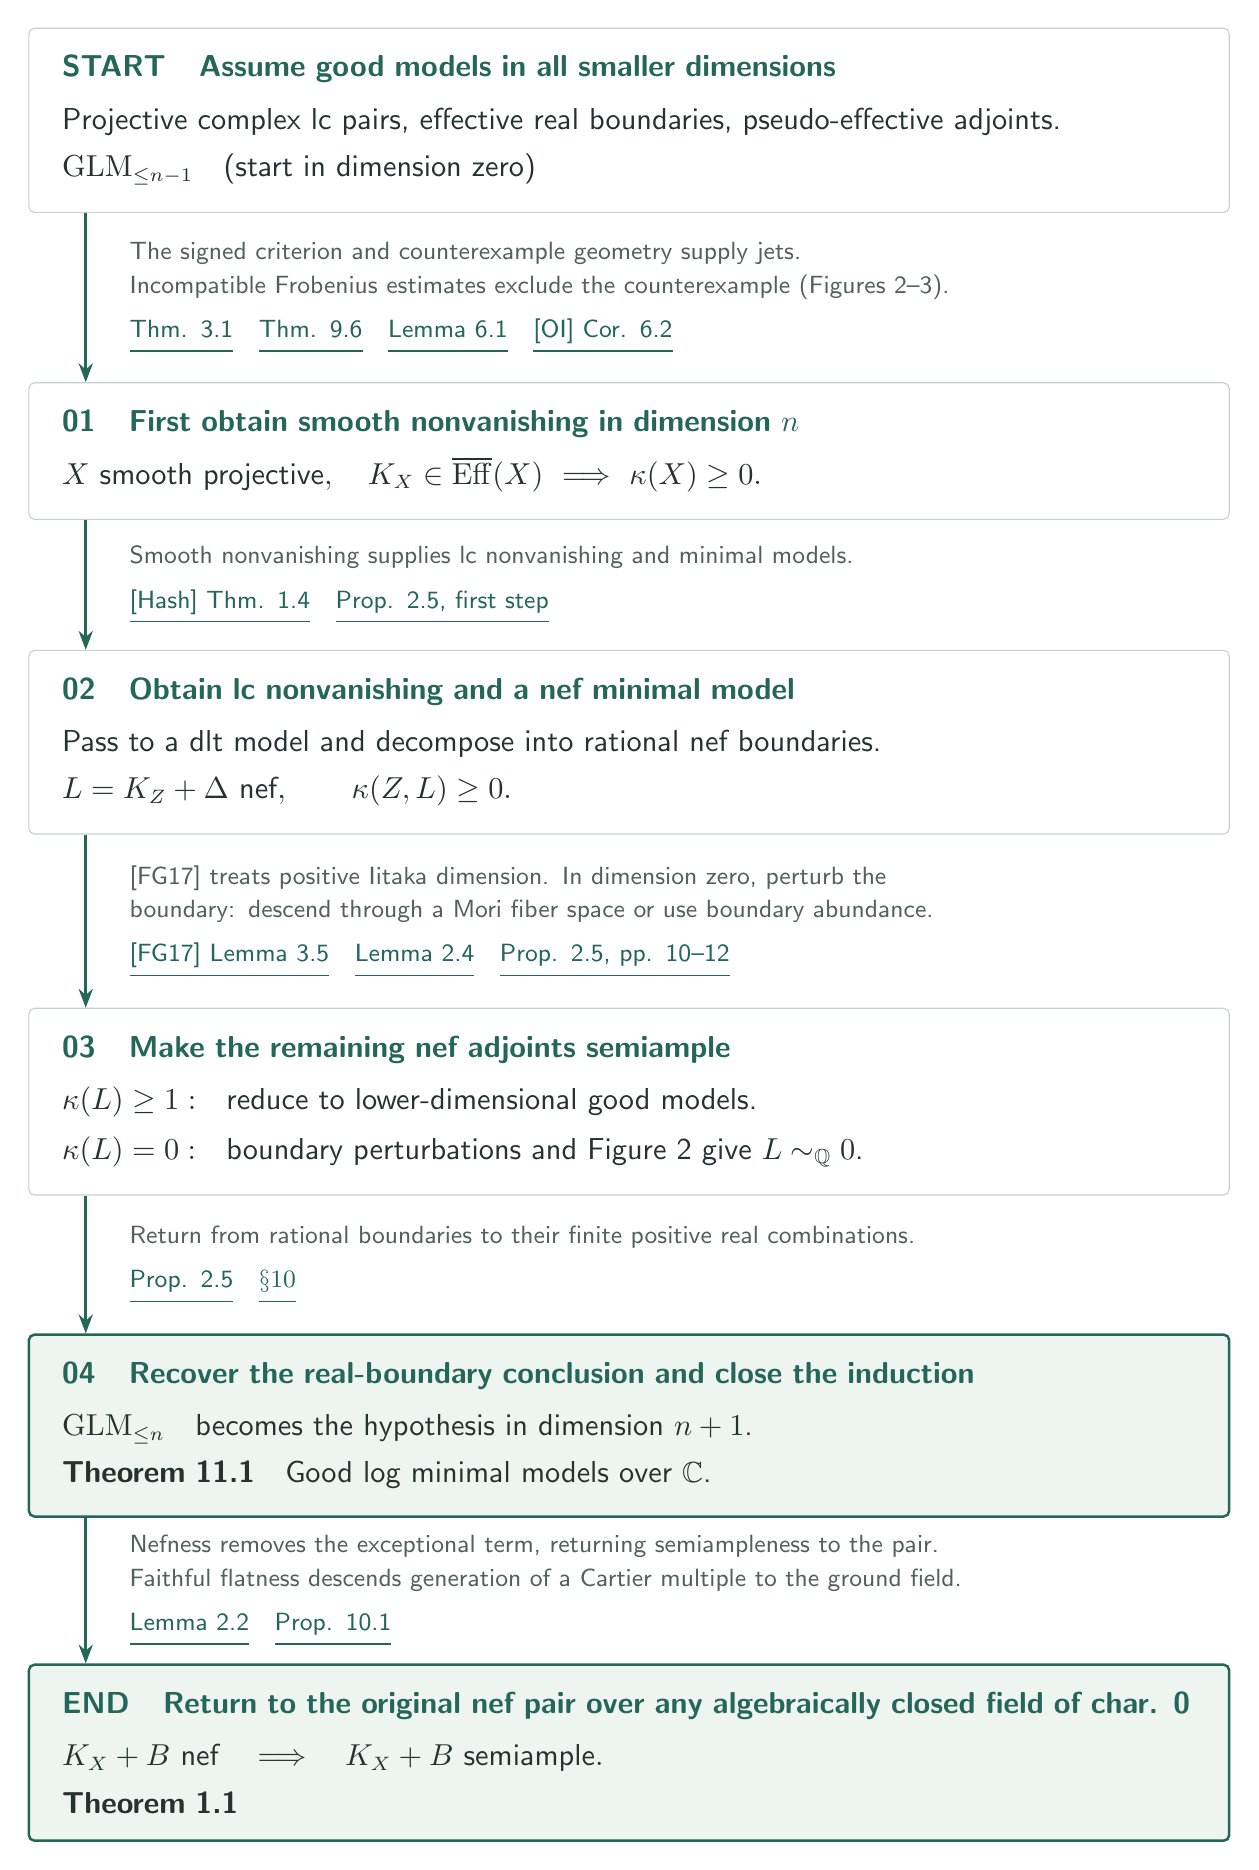
\begin{tikzpicture}
\node[card] (start) {\heading{START}{低次元の「良い極小モデル」を仮定する}{Assume good models in all smaller dimensions}
\Tx{複素射影的 lc 対・有効な実係数境界・擬有効な随伴因子。}{Projective complex lc pairs, effective real boundaries, pseudo-effective adjoints.}\\[3pt]
$\mathrm{GLM}_{\leq n-1}$\quad\Tx{（次元0から開始）}{(start in dimension zero)}};
\node[card,below=2.15cm of start] (nv) {\heading{01}{まず、次元 $n$ の滑らかな非消滅を得る}{First obtain smooth nonvanishing in dimension $n$}
$X\text{ smooth projective},\quad K_X\in\Eff(X)\ \Longrightarrow\ \kappa(X)\geq0.$};
\flow{start}{nv}{\Tx{符号付き境界の判定と反例の幾何からジェットを構成。\\Frobenius による相反する評価で反例を排除する（図2・3）。}{The signed criterion and counterexample geometry supply jets.\\Incompatible Frobenius estimates exclude the counterexample (Figures 2--3).}\\[4pt]
\LA{12}{Thm. 3.1}\quad\LA{69}{Thm. 9.6}\quad\LA{30}{Lemma 6.1}\quad\OI{40}{[OI] Cor. 6.2}}
\node[card,below=1.65cm of nv] (nef) {\heading{02}{lc 対の非消滅と、nef な極小モデルを得る}{Obtain lc nonvanishing and a nef minimal model}
\Tx{実係数 lc 対を dlt モデルへ。有理係数 nef 境界に分解する。}{Pass to a dlt model and decompose into rational nef boundaries.}\\[3pt]
$L=K_Z+\Delta\ \text{nef},\qquad\kappa(Z,L)\geq0.$};
\flow{nv}{nef}{\Tx{滑らかな非消滅から、実係数 lc 対の非消滅と極小モデル存在へ。}{Smooth nonvanishing supplies lc nonvanishing and minimal models.}\\[4pt]
\Hash{1}{[Hash] Thm. 1.4}\quad\LA{9}{Prop. 2.5, first step}}
\node[card,below=2.2cm of nef] (good) {\heading{03}{残った nef 随伴因子を半豊富にする}{Make the remaining nef adjoints semiample}
$\kappa(L)\geq1:$\quad\Tx{低次元の良いモデルへ帰着。}{reduce to lower-dimensional good models.}\\[4pt]
$\kappa(L)=0:$\quad\Tx{境界の摂動と図2を使い、$L\sim_{\mathbb Q}0$。}{boundary perturbations and Figure 2 give $L\sim_{\mathbb Q}0$.}};
\flow{nef}{good}{\Tx{正の小平次元は [FG17]。0 の場合は、摂動後の擬有効性で分岐し、\\Mori ファイバー空間への降下、または境界上の abundance を使う。}{[FG17] treats positive Iitaka dimension. In dimension zero, perturb the\\boundary: descend through a Mori fiber space or use boundary abundance.}\\[4pt]
\FGring{5}{[FG17] Lemma 3.5}\quad\LA{9}{Lemma 2.4}\quad\LA{10}{Prop. 2.5, pp. 10--12}}
\node[result,below=1.75cm of good] (induction) {\heading{04}{実係数の結論を得て、帰納法を閉じる}{Recover the real-boundary conclusion and close the induction}
$\mathrm{GLM}_{\leq n}$\quad\Tx{を次元 $n+1$ の仮定へ。}{becomes the hypothesis in dimension $n+1$.}\\[3pt]
\textbf{Theorem 11.1}\quad\Tx{複素数体上の良い対数的極小モデル。}{Good log minimal models over $\mathbb C$.}};
\flow{good}{induction}{\Tx{有理係数での半豊富性を、有限個の正の実結合へ戻す。}{Return from rational boundaries to their finite positive real combinations.}\\[4pt]\LA{9}{Prop. 2.5}\quad\LA{72}{$\S10$}}
\node[result,below=1.85cm of induction] (end) {\heading{END}{元の nef 対へ戻し、任意の標数0の代数閉体へ}{Return to the original nef pair over any algebraically closed field of char. 0}
$K_X+B\ \text{nef}\quad\Longrightarrow\quad K_X+B\ \text{semiample}.$\\[3pt]\textbf{Theorem 1.1}};
\flow{induction}{end}{\Tx{nef 性で比較式の例外項を消し、元の対に半豊富性を降ろす。\\Cartier 倍の評価写像の全射性を忠実平坦性で降ろし、基礎体を変更。}{Nefness removes the exceptional term, returning semiampleness to the pair.\\Faithful flatness descends generation of a Cartier multiple to the ground field.}\\[4pt]\LA{8}{Lemma 2.2}\quad\LA{72}{Prop. 10.1}}
\end{tikzpicture}

\end{document}
